%----------------------------------------------------------------
%
%  File    :  chapter4.tex
%
%  Authors :  Michael Fuska, FH Campus Wien, Austria
% 
%  Created :  08 Feb 2016
% 
%  Changed :  
% 
%----------------------------------------------------------------
\chapter{Mobile Apple Betriebssystem iOS}
\label{ch:iOS}
%------------------------------------------------------------------------------
%---------------------------------- iOS Grundlagen
\section{iOS Grundlagen}
\label{sec:iOSGrundlage}

Das mobile Apple Betriebssystem iOS basiert auf dem Desktop Betriebssystem des Mac OS X. Darwin ist ein frei erhältliches, Linux basiertes Betriebssystem. Dieses Betriebssystem stellt die Grundlage für das Mac OS X dar. Der Kernel des Mac OS X ist der XNU-Kernel mit entsprechenden Adaptionen für das Mac OS X und dem mobilen Betriebssystem iOS.\par 
\begin{figure}[hp!]
        \centering
                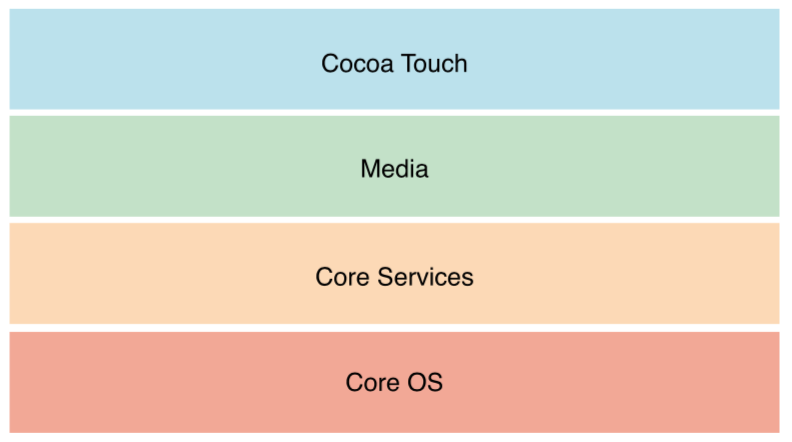
\includegraphics[height=5cm]{Bilder/Chapter3_SystemArchitektur}
        \caption{iOS Software Layer (\cite{Apple[5]} S. 9)}
        	\label{fig:iOS Software Layer}
\end{figure}
Die abgebildeten Schichten zeigen das abstrahierte iOS Betriebssystem. Der grösste Unterschied zwischen Mac OS X und iOS liegt im Cocoa Touch Layer.
\begin{description}
\item[Folgende Anforderungen werden an das iOS Software Layer Modell gestellt]~\par
	\begin{itemize}
		\item Sicherstellungen der \textbf{Datenintegrität}
		\item Gewährleistung der \textbf{Informationsvertraulichkeit}
		\item Sicherstellung der \textbf{User- und/oder Applikation Authentizität}
		\item Gewährleistung der \textbf{Daten/Informationsverbindlichkeit}
	\end{itemize}
\end{description}
%------------------------------------------------------------------------------
%---------------------------------- iOS Software Layer
\section{iOS Software Layer}
\label{sec:iOSSWLayer}
%---------------------------------- Core OS
\subsection{Core OS Layer}
\label{sec:CoreLayer}
Der \textbf{Core OS Layer} beinhaltet alle \textit{\glqq Low Level Features\grqq}. Auf diesen Layer bauen alle anderen \textit{\glqq Frameworks\grqq{}} auf. Der iOS Applikationsentwickler kommt mit diesem Layer nur dann in Berührung, wenn dieser sich mit der Sicherheit und mit der Hardware-Kommunikation beschäftigt. 
\begin{description}
	\item[\parbox{\textwidth} {Das Core OS Layer Framework beinhaltet folgende Frameworks}]~\par
	\begin{itemize}
		\item Accelerate Framework
		\item Core Bluetooth Framework
		\item External Accessory Framework
		\item Generic Security Service Framework
		\item Lost Authentication Framework
		\item Network Extension Framework
		\item Security Framework
		\item System
		\item 64-Bit Support
	\end{itemize}
\end{description}
 (Vgl. \cite{Apple[6]} S.49-52) 
 
%---------------------------------- Core Service
\subsection{Core Service Layer}
\label{sec:CoreServiceLayer}		
Der \textbf{Core Service Layer} beinhaltet die fundamentalen System Services. Dieser Layer wird unterteilt in \textit{\glqq High Level Feature\grqq{}} und \textit{\glqq Core Service Frameworks\grqq{}}.

\begin{description}
    \item[\parbox{\textwidth} {Die High Level Features dieses Layers sind}]~\par
	\begin{itemize}
		\item \textbf{Peer-to-Peer Services}
		\item \textbf{iCloud Storage}
		\item \textbf{Block Objects}
		\item \textbf{Data Protection}
		\item \textbf{File-Sharing Support}
		\item \textbf{Grand Central Dispatch}
		\item \textbf{In-App Purchase}
		\item \textbf{SQLite}
		\item \textbf{XML Support} 
	\end{itemize}
\end{description}

\newpage
\begin{description}	
	\item[\parbox{\textwidth} {Das Core Service Layer Framework beinhaltet folgende Frameworks}]~\par
	\begin{multicols}{2}
	\begin{itemize}
		\item Accounts Frameworks
		\item Address Book Framework
		\item Ad Support Framework
		\item CFNetwork Framework
		\item CloudKit Framework
		\item Core Data Framework
		\item Core Foundation Framework
		\item Core Location Framework
		\item Core Media Framework
		\item Core Motion Framework
		\item Core Telephony Framework
		\item EvenKit Framework
		\item Foundation Framework
		\item HealthKit Framework
		\item HomeKit Framework
		\item JavaScript Framework
		\item Mobile Core Services Framework
		\item Multipeer Connectivity Framework
		\item NewStandKit Framework
		\item PassKit Framework
		\item Quick Look Framework
		\item Safari Services Framework
		\item Social Framework
		\item StoreKit Framework
		\item System Configuration Framework
		\item WebKit Framework
	\end{itemize}
	\end{multicols}
\end{description}
(Vgl. \cite{Apple[6]} S.36-48)
%---------------------------------- Media Layer
\subsection{Media Layer}
\label{sec:MediaLayer}		
Der \textbf{Media Layer} beinhaltet alle Technologien zur Darstellung von Grafik, Video und das Abspielen von Tönen. Dieser Layer ist verantwortlich für das Design und den Sound der iOS Apps. 

\begin{description}
	\item[Dieser Layer stellt folgende Technologien zur Verfügung]~\par
    \begin{itemize}
		\item \textbf{Graphics Technologies}
		\item \textbf{Audio Technologies}
		\item \textbf{Video Technologies}
		\item \textbf{AirPlay}
    \end{itemize}

    \item[\parbox{\textwidth} {Das Media Layer Framework beinhaltet folgende Frameworks}]~\par
	\begin{multicols}{2}
	\begin{itemize}
		\item Assets Library Framework
		\item AV Foundation Framework
		\item AVKit Framework
		\item CoreAudioKit Framework
		\item Core Graphics Framework
		\item Core Image Framework
		\item Core Text Framework
		\item Core Video Framework
		\item Game Controller Framework
		\item GLKit Framework
		\item Image I/O Framework
		\item Media Accessibility Framework
		\item Media Player Framework
		\item Metal Framework
		\item OpenGL ES Framework
		\item Photos Framework
		\item Photos UI Framework
		\item Quartz Core Framework
		\item SceneKit Framework
		\item SpriteKit Framework
         \end{itemize}
	\end{multicols}
\end{description}
(Vgl. \cite{Apple[6]} S.23-35)
%---------------------------------- Cocoa Touch Layer
\subsection{Cocoa Touch Layer}
\label{sec:CocoaTouchLayer}
Enthält die wichtigsten Frameworks, um iOS Applikationen zu entwickeln. Dieser
Layer stellt die Basis Applikation Infrastruktur und folgende Key Technologien zur Verfügung
	\begin{itemize}
		\item \textbf{Multitasking}
		\item \textbf{Touch-based Input}
		\item \textbf{Push Notification}
		\item \textbf{High-level System Service}	
	\end{itemize}
\begin{description}
\item[Folgende Features sind in Cocoa Touch Layer enthalten]~\par
	\begin{multicols}{2}
	\begin{itemize}
		\item App Extentision
		\item Handoff
		\item Document Picker
		\item AirDrop
		\item TextKit
		\item UIKit Dynamics
		\item Multitasking
		\item Auto Layout
		\item Storyboards
		\item UI State Preservation
		\item Apple Push Notification Service
		\item Local Notifications
		\item Gesture Recognizers
		\item Standard System View Controllers
         \end{itemize}
	\end{multicols}	
	 \item[\parbox{\textwidth} {Das Cocoa Touch Layer Framework beinhaltet folgende Frameworks}]~\par
	\begin{multicols}{2}
	\begin{itemize}
		\item Address Book UI Framework
		\item EventKit UI Framework
		\item GameKit
		\item  Framework
		\item iAd Framework
		\item MapKit Framework
		\item Message UI Framework
		\item Notification Center Framework
		\item PushKit Framework
		\item Twitter Framework
		\item UIKit Framework
         \end{itemize}
	\end{multicols}
\end{description}
(Vgl. \cite{Apple[6]} S.12-22)

%---------------------------------- iOS Device Security Architektur
\pagebreak
\section{iOS Device Security Architektur}
\label{sec:iOSSecArchitektur}

Die in diesem Kapitel beschrieben Sicherheitsmechanismen beziehen sich auf alle iOS Produkte ab dem Apple A7 Prozessor. Alle Prozessoren vor dem Apple A7 besitzen keinen Coprozessor mit Secure Enclave (siehe Abb. \ref{fig:iOSSecurityArchitekturiOS7}).\par

\begin{figure}[htb]
  \begin{minipage}{0.6\textwidth} 
  Der Sicherheitsmechanismus des iOS Device unterteilt sich in zwei Ebenen. 
  		\begin{description}
   			\item[ iOS Sicherheitsebenen]~\par
         		\begin{enumerate}	
				\item  \textbf{iOS Software}
					\begin{enumerate}
       						\item File System
         					\item OS Partition
						\item User Partition (verschlüsselt)
						\item App Sandbox
						\item Data Protection Class
      					\end{enumerate}
      				\item  \textbf{iOS Hardware und Firmware}~\par
					\begin{enumerate}
       						\item Kernel
						\begin{enumerate}
						\item Secure Enclave
						\item Secure Element
         					\end{enumerate}	
						\item Crypto Engine
						\item Device Key
						\item Group Key
						\item Apple Root Certificate
      					\end{enumerate}
			\end{enumerate}
   		\end{description}
Die iOS Sicherheit passiert auf einer Kombination von Software, Hardware und Service, um ein Maximum an Sicherheit zu erreichen (vgl. \cite{Apple[4]} S.4).
	\end{minipage}
	\hfil
	\begin{minipage}{0.4\textwidth}
		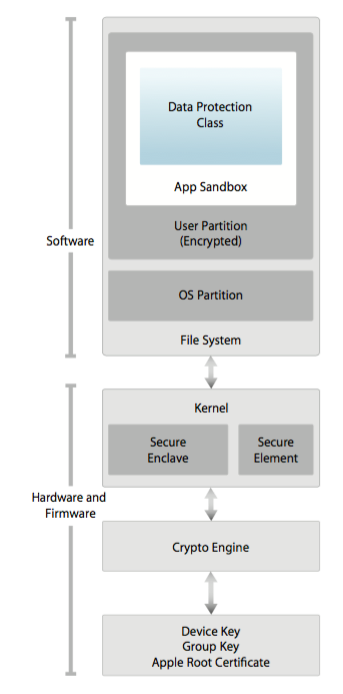
\includegraphics[width=\textwidth]{Bilder/Chapter3_SecArchitektur}
		\caption {iOS Security Architektur (\cite{Apple[4]} S.4)}
        \label{fig:iOS Security Architektur}
	\end{minipage}
\end{figure}
		    	
%---------------------------- System Security
\subsection{System Security}
\label{sec:SystemSec}
Die \textbf{System Security} von einem iOS Device ist so kon­zep­ti­o­nie­rt, dass die Software und Hardware sicher über alle Kernkomponenten des Devices ist. Dies beinhaltet den sicheren Boot Prozess (siehe Kap. \ref{sec:SecBootChain}), die Software Updates und die \textit{\glqq Secure Enclave\grqq{}} (siehe Kap. \ref{sec:HardwareSecProtection}). Alle diese Maßnahmen dienen dazu sicherzustellen, dass nur vertrauenswürdige Applikationen auf dem iOS Device ausgeführt werden können.\par 

Die enge Verbindung zwischen Hardware und Software eines iOS Gerätes gewährleistet, dass alle Komponenten des Systems vertrauenswürdig sind, sowohl die Software als auch die Hardware (vgl. \cite{Apple[4]} S.5).

\vspace*{1cm}

\begin{description}
\item[Apple führt unter dem Kapitel System Security folgende Features an]~\par
	%\begin{multicols}{2}
	\begin{itemize}
		\item Secure Boot Chain (siehe Kap. \ref{sec:SecBootChain})
 		\item System Software Authorization (siehe Kap. \ref{sec:SigningProcess})
 		\item Secure Enclave (siehe Kap. \ref{sec:HardwareSecProtection})
 		\item Touch ID (siehe Kap. \ref{sec:Passcode})
        \end{itemize}
	%\end{multicols}
\end{description}
(Vgl. \cite{Apple[4]} S.5-9)

%--------------------------- Encryption und Daten Sicherheit
\subsection{Encryption und Daten-Sicherheit}
\label{sec:DataEnc}

Das iOS Device unterstützt standardmäßig eine Verschlüsselung für persönliche Daten und Unternehmensdaten. Die Sicherheitsinfrastruktur des iOS Devices ist so aufgebaut, dass selbst wenn ein Teil des Betriebssystem kompromittiert ist, die anderen Bereiche des iOS Devices weiterhin sicher vor unerlaubtem Zugriff sind. \par
Dies ist besonders für Unternehmen wichtig, da dadurch gewährleistet wird, dass vertrauliche Unternehmensdaten nicht gelesen werden können. Weitere iOS Features stellen sicher, dass selbst bei Diebstahl oder Verlust des iOS Devices die Daten sicher sind. Alle diese Features sind in der Standardkonfiguration des mobilen Betriebssystems aktiv gesetzt.

\begin{description}
\item[\parbox{\textwidth} {Apple führt unter dem Kapitel Encryption und Daten-Sicherheit folgende Features an}]~\par
	\begin{itemize}
		\item \textbf{Hardware Security Features} (siehe Kap. \ref{sec:HardwareSecProtection})
 		\item \textbf{File Datenschutz} (siehe Kap. \ref{sec:DataProtection})
 		\item \textbf{Passcodes} (siehe Kap. \ref{sec:Passcode})
 		\item \textbf{Data Protection Classes}  (siehe Kap. \ref{sec:HardwareSecProtection})
		\item \textbf{Keychain Data Protection} (siehe Kap. \ref{sec:HardwareSecProtection})
	\end{itemize}
\end{description}
(Vgl. \cite{Apple[4]} S.10-17)

%------------------------------ Applikation Security
\subsection{Applikation Security}
\label{sec:AppSec}
Für das Betriebssystem beinhalten die zu installierenden Apps das größte Sicherheitsrisiko. Das Verhalten des Betriebssystems kann durch eine App negativ beeinflusst werden. Es kann die Sicherheit und die Verfügbarkeit des iOS Devices negativ beeinflusst werden. Des weiteren kann die Integrität der Benutzerdaten durch eine unsicher programmierte  App gefährdet werden.
\begin{description}
\item[\parbox{\textwidth} {Apple führt unter dem Kapitel Applikation Security folgende Features an}]~\par
	\begin{itemize}
		\item \textbf{App Code signing} (siehe Kap. \ref{sec:SigningProcess}) 
		\item \textbf{Runtime process security} (siehe Kap. \ref{sec:MemoryProtection})
		\item \textbf{Extensions}
		\item \textbf{App Groups} (siehe Kap. \ref{sec:Sandbox})
		\item \textbf{Data Protection in Apps} (siehe Kap. \ref{sec:SystemSec})
    \end{itemize}
\end{description}
(Vgl. \cite{Apple[4]} S.18-26)

%------------------------------ Network Security
\subsection{Netwerk Sicherheit}
\label{sec:NetworkSec}
Die \textbf{ Netzwerk Sicherheit} ist ein wichtiger Bestandteil des Sicherheitskonzepts und ergänzt die integrierten iOS Sicherheitsmechanismen. Die integrierten Sicherheitsmechanismen des mobilen Betriebssystems von Apple dienen dazu, die Daten auf dem Device zu schützen. Die Anforderungen an ein mobiles Device haben sich in den letzten Jahren dahin gehend verändert, dass der Zugriff auf externe Daten geschützt vorgenommen werden kann. Dieser Zugriff muss so abgesichert sein, dass die Datenübertragung sicher ist und die Usability des Produktes nicht eingeschränkt ist. Es werden Netzwerksicherheit-Protokolle und -Architekturen für eine authentifizierte, autorisierte und verschlüsselte Kommunikation verwendet.
\begin{description}
\item[\parbox{\textwidth} {Ein iOS Device verfügt über folgende Netzwerksicherheit-Protokolle und -Architekturen
an}]~\par
	\begin{itemize}
		\item \textbf{Virtual Private Network (VPN)}
 		\item \textbf{Single Sign-on}
 		\item \textbf{Internet Protocol Security (IPsec)}
 		\item \textbf{Transport Layer Security (TLS)} %(siehe Kap. \ref{sec:TLS})
		\item \textbf{Datagram Transport Layer Security (DTLS)}
        \end{itemize}
\end{description}
Weiters werden die neuersten Standards für WLAN, Bluetooth und Mobilfunk-Verbindungen verwendet (vgl. \cite{Apple[4]} S.27-30).

%------------------------------ Apple Pay ----------------------------------
\subsection{Apple Pay}
\label{sec:ApplePay}

\textbf{Apple Pay} ist das interne Apple Zahlungssystem für mobile Geräte. Die Kommunikation findet über NFC statt. Neben NFC ist die App \textit{\glqq Wallet\grqq{}} Teil des Apple Pay Produkts.

\newpage
\begin{description}
\item[\parbox{\textwidth} {Folgende Komponenten gehören zu dem Apple Pay Produkt}]~\par
	\begin{itemize}
		\item \textbf{Secure Elements:} \\
        Alle Secure Elements erfüllen den Industriestandard. Der zertifizierte Chip wird auf einer Java Card Plattform ausgeführt. Diese Elemente erfüllen den Finanzindustrie Standard. 
 		\item \textbf{Near Field Communication (NFC) Controller:} \\
        Der NFC Controller und die NFC Kommunikation Protokolle sind für die Kommunikation zwischen den Anwendungsprozessoren und Secure Elementen zuständig.
 		\item \textbf{Wallet:} \\
        Die Wallet App ist für die Verwaltung der Kreditkarten und Debitkarten verantwortlich. 
            \begin{description}
                \item[\parbox{\textwidth} {Diese App ermöglicht es dem User}]~\par
                \begin{itemize}
                    \item die Kartendaten,
                    \item den Kartenaussteller,
                    \item die durchgeführten Transaktionen der einzelnen Karten und
                    \item vieles mehr
                \end{itemize}
            \end{description} 
        \textbf{abzuspeichern und anzuzeigen.}
        
 		\item \textbf{Secure Enclave:}\\
        Die Secure Enclave ist für den Authentifizierungsprozess einer Finanztransaktion zuständig. Des weiteren werden in der Secure Enclave die Touch-ID Fingerabdrücke gespeichert.	
        \end{itemize}
\end{description}
(Vgl. \cite{Apple[4]} S.31-37)

%------------------------------ Internet services
\subsection{Internet Services}
\label{sec:InternetServices}

Apple hat sich die Prämisse gestellt, stabile Applikationen mit guter Benutzbarkeit für den Benutzer zu entwickeln. 
\begin{description}
    \item[\parbox{\textwidth} {Beispiele für solche internen iOS Apps sind }]~\par
    \begin{itemize}
       \item iMessage,
       \item Facetime,
       \item iCloud und 
       \item iCloud Keychain.
    \end{itemize}
\end{description} 

Apple stellt den Entwicklern von Internet Diensten die Frameworks zur Verfügung, die auch für interne Apple Apps verwendet werden. Natürlich gelten für Internet Dienste die selben Sicherheitsziele, wie für die internen Apple Produkte. Diese Ziele beinhalten den \textit{\glqq sicheren Umgang mit den persönlichen Daten der Benutzer\grqq{}} sowie \textit{\glqq den Schutz vor nicht autorisiertem Zugriff auf die persönlichen Daten des Benutzers\grqq{}} und \textit{\glqq anderer Dienstleistungen\grqq{}}. Jeder Dienst verwendet eine eigene leistungsstarke Sicherheitsarchitektur ohne die Benutzerfreundlichkeit des gesamten iOS Devices zu beeinträchtigen (vgl. \cite{Apple[4]} S.38-49).

\begin{description}
    \item[\parbox{\textwidth} {Dies sind die Mainfeatures des Apple Internet Service}]~
    \begin{itemize}
        
        \item \textbf{Apple-ID:}\\
        Die \textbf{Apple-ID} ist Teil des persönlichen Apple-Accounts, der zusammen mit dem \textit{\glqq Password\grqq{}} den Zugriff auf die Apple Service ermöglicht. 
        
        \item \textbf{iCloud:} \\
        Die \textbf{iCloud} ist der Apple Online-Dienst zum Speichern und Synchronisieren von Daten/Konfigurationen. 
        
        \item \textbf{iCloud Keychain:}\\
        Die \textbf{iCloud Keychain} ist das Apple Online \textit{\glqq Password Management System\grqq{}}. \begin{description}
                \item[\parbox{\textwidth} {Das Password Management System dient zum Speichern von}]~\par
                    \begin{itemize}
                        \item systemübergreifenden Passwörtern,
                        \item Login Daten,
                        \item WLAN-Zugangsdaten und 
                        \item Kreditkartendaten.
                    \end{itemize}
                \end{description} 
 
        \item \textbf{Continuity:}\\
        Darunter versteht Apple das Verteilen von Informationen und Services über mehrere iOS Devices. 
        \begin{description}
        \item[\parbox{\textwidth} {Beispiele für Continuity sind}]~\par
            \begin{itemize}
                \item Die Anrufannahme auf unterschiedlichen iOS Devices
                \item Die Möglichkeit, Nachrichten auf unterschiedlichen iOS Devices zu lesen und zu schreiben.
                \item Das Verteilen von Dateien auf iOS Devices.
            \end{itemize}
        \end{description}  
    \end{itemize}
\end{description}

%------------------------------ Device Controls
\subsection{Device Controls}
\label{sec:DeviceControl}

Der \textbf{Device Control} Mechanismus von Apple hat die Aufgabe, flexible Sicherheitsrichtlinien und Konfigurationen umzusetzen. Eine weitere Rahmenbedingung ist, dass die Konfiguration der Geräte leicht umsetzbar und verwaltbar ist.\par 
 Für Unternehmen bringt dies den Vorteil mit sich, dass Sicherheitsrichtlinien und Konfigurationen auf mehrere iOS Geräte verteilt werden können. Dadurch können Firmen sicherstellen, dass alle Geräte die selben Einstellungen besitzen. Weiters ermöglicht es Mitarbeitern ihre eigenen Geräte im Unternehmen zu verwenden (BYOD). 

\begin{description}
    \item[\parbox{\textwidth} {Dies sind die Mainfeature des Apple Device Control Service} ]~\par
    \begin{multicols}{2}
    \begin{itemize}
        \item Passcode Sicherheit
        \item iOS pairing model
        \item Konfigurationsverteilung
        \item Mobile Device Management(MDM)
        \item Device Enrollment Program
        \item Device restriction
        \item Apple Configurator
        \item Supervised-only restrictions
        \item Remote wipe
        \item Find My iPhone and 
        \item Activation Lock
    \end{itemize}
    \end{multicols}
\end{description}
(Vgl. \cite{Apple[4]} S.50-55)
%----------------------------- Privacy Controls

\subsection{Datenschutzkontrolle}
\label{sec:PrivacyControls}
Das mobile Betriebssystem von Apple verfügt über zahlreiche integrierte Steuerelemente und Optionen. Diese iOS Einstellungen ermöglichen es dem Benutzer zu entscheiden, wie mit seinen persönlichen Daten umgegangen werden soll. Dies inkludiert, welche App Zugriff auf welche Informationen bekommen soll. 

\begin{description}
    \item[\parbox{\textwidth} {Folgende Daten werden für die Ortung des Users verwendet (Location Service) }]~\par
    \begin{itemize}
        \item GPS Daten,
        \item Bluetooth Daten,
        \item öffentliche WLAN-Hotspots
        \item Mobilfunkmasten
    \end{itemize}
    Der User hat die Möglichkeit, mit Hilfe von iOS Einstellungen zu definieren, welche App welche Location Daten verwenden kann.
    \item[\parbox{\textwidth} {Zu den persönlichen User-Daten zählen}]~\par
    \begin{multicols}{2}
    \begin{itemize}
        \item Kontakte
        \item Kalender
        \item Erinnerungen
        \item Fotos
        \item Aktivitätsdaten
        \item Accounts sozialer Netzwerke
        \item Mikrofon
        \item Kamera
        \item Bluetooth-Freigabe
    \end{itemize}
      \end{multicols}
\end{description}
(Vgl. \cite{Apple[4]} S.56, \cite{Apple[8]} S.49)